\documentclass[10pt]{beamer}

\usepackage{fontspec}
\setmainfont{Ubuntu}[]
\setsansfont{Ubuntu}[]
\setmonofont{Ubuntu Mono}[]

\usepackage{graphicx}
\graphicspath{ {../img/} }

\usepackage[absolute,overlay]{textpos} % [showboxes]
\usepackage{listings}

\beamertemplatenavigationsymbolsempty

\lstset{
  language=ML,
  keywordstyle=\color{blue},
  backgroundcolor=\color{lightgray}
}

\title{Немного истории}

\begin{document}

\begin{frame}
  \frametitle{Немного истории}
  \textbf{Предыстория}: начало ХХ века.
  \par \bigskip
  \textbf{История Эрланг}: c 1985 по настоящее время.
  \par \bigskip
  \textbf{История Эликсир}: c 2012 по настоящее время.
\end{frame}


\begin{frame}
  \frametitle{Предыстория: начало ХХ века.}
  \begin{textblock*}{70pt}(30pt,60pt)
    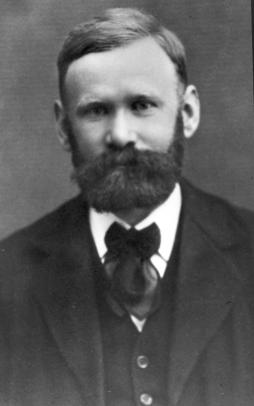
\includegraphics{agner_krarup_erlang}
  \end{textblock*}
  \begin{textblock*}{220pt}(120pt,65pt)
    \textbf{Агнер Краруп Эрланг}
    \par \bigskip
    Датский математик, статистик и инженер.
    \par \bigskip
    Научный подход к изучению трафика в телефонных сетях.
    \par \bigskip
    Автор "Теории массового обслуживания".
  \end{textblock*}
\end{frame}

\begin{frame}
  \frametitle{Теория массового обслуживания}
  Она же теория очередей (Queueing theory).
  \par \bigskip
  Математическая модель для оценки пропускной способности телекоммуникационных сетей.
\end{frame}

\begin{frame}
  \frametitle{Теория массового обслуживания}
  применяется в телекоммуникационных системах,
  \par \bigskip
  а также:
  \begin{itemize}
  \item в логистике,
  \item в управлении автомобильным движением,
  \item на конвейерном производстве,
  \item при проектировании складов и больниц.
  \end{itemize}
\end{frame}

\begin{frame}
  \frametitle{Эрланг}
  Язык Эрланг родился в шведской компании \textbf{Эрикссон} (\textbf{Ericsson}).
  \par \bigskip
  Крупный поставщик телекомуникационного оборудования и~услуг.
\end{frame}

\begin{frame}
  \frametitle{Эрланг}
  Для телеком индустрии характерны:
  \begin{itemize}
  \item сложное оборудование,
  \item сложный софт,
  \item большой трафик,
  \item жесткие требования по доступности сервиса.
  \end{itemize}
\end{frame}

\begin{frame}
  \frametitle{Ericsson’s Computer Science Laboratory}
  Задача:
  \par \bigskip
  Найти более эффективные средства разработки софта для железа и сервисов компании.
\end{frame}

\begin{frame}
  \frametitle{Ericsson’s Computer Science Laboratory}
  Прототипы телеком-приложений на разных языках:
  \begin{itemize}
  \item функциональные языки ML и Miranda,
  \item многопоточные языки ADA, Modula и Chill,
  \item логический язык Prolog,
  \item объектно-ориентированный Smalltalk.
  \end{itemize}
\end{frame}

\begin{frame}
  \frametitle{Ericsson’s Computer Science Laboratory}
  Ни один язык не имеет нужных возможностей.
  \par \bigskip
  Главная проблема -- многопоточность.
\end{frame}

\begin{frame}
  \frametitle{Эрланг}
  \begin{textblock*}{75pt}(30pt,60pt)
    
\includegraphics[scale=2.8]{erlang_logo}
  \end{textblock*}
  \begin{textblock*}{220pt}(120pt,70pt)
    В итоге лаборатория решила разработать свой язык~программирования.
  \end{textblock*}
\end{frame}

\begin{frame}
  \frametitle{Эрланг}
  1998 год: Эрланг выпушен в open source.
  \par \bigskip
  2002 год: \textbf{Ejabberd} -- первый крупный open source проект.
  \par \bigskip
  Стал основой для большинства IM (Instant Messaging) систем,
  \par \bigskip
  в т.ч. для широко известного \textbf{WhatsApp}.
\end{frame}

\begin{frame}
  \frametitle{Эрланг}
  2006 год: поддержка симметричной мультипроцессорности (SMP).
  \par \bigskip
  Эрланг научился эффективно использовать все имеющиеся в~системе процессорные ядра.
\end{frame}

\begin{frame}
  \frametitle{Эрланг}
  У IT-индустрии появилась потребность
  разрабатывать многопоточные программы.
  \par \bigskip
  Возник интерес к функциональному программированию вообще,
  и к Эрланг в частности.
\end{frame}

\begin{frame}
  \frametitle{Интерес к ФП}
  Этот интерес проявился в двух направлениях:
  \begin{itemize}
  \item стали шире использоваться ФП языки;
  \item популярные языки начали заимствовать идеи ФП и реализовывать их у себя.
  \end{itemize}
\end{frame}

\begin{frame}
  \frametitle{Эликсир}
  \begin{textblock*}{75pt}(30pt,60pt)
    
\includegraphics[scale=2.9]{elixir_logo}
  \end{textblock*}
  \begin{textblock*}{220pt}(120pt,60pt)
    Эликсир создан в 2012 году в компании Plataformatec.
    \par \bigskip
    Его автор -- \textbf{Жозе Валим}.
    \par \bigskip
    Один из основных разработчиков фреймворка Ruby on Rails
    и сооснователь компании Plataformatec.
  \end{textblock*}
\end{frame}

\begin{frame}
  \frametitle{Эликсир}
  Позаимствовал идеи из Ruby, Clojure и Эрланг.
  \par \bigskip
  Развивался под влиянием Ruby и Ruby on Rails.
  \par \bigskip
  Система макросов заимствована из Clojure.
  \par \bigskip
  Унаследовал все возможности Эрланг и его виртуальной машины.
\end{frame}

\begin{frame}
  \frametitle{Эликсир}
  2014 год: Эликсир 1.0
  \par \bigskip
  2015 год: Ecto 1.0 и Phoenix 1.0
\end{frame}

\end{document}
